\documentclass[hidelinks,a4paper, 12pt]{article}
\usepackage[french]{babel}
\usepackage[utf8]{inputenc}
\usepackage[T1]{fontenc}
\usepackage{lmodern}
\usepackage{graphicx}
\usepackage{hyperref}
\usepackage{listings}
\usepackage{color}
\usepackage{svg}
\usepackage{cleveref}
\usepackage{subfig}
\usepackage{gensymb}
\usepackage{slashbox}
\usepackage[titletoc,title]{appendix}
\lstset{language=C,rangeprefix=//---------------,rangesuffix=----------------,includerangemarker=false,columns=spaceflexible,extendedchars=true,showspaces=false,showstringspaces=false,inputencoding=ansinew,tabsize=4,frame=shadowbox,morecomment=[is]{\#ifdef}{\#endif},morecomment=[is]{/*}{*/}}
\title{Lecture et rédaction scientifiques: \\Skip-lists }
\author{Steve Zaretti}

\begin{document}
	
	\maketitle
	\newpage
	\tableofcontents
	\newpage
	
	\section{Introduction}
	En informatique, il est courant de vouloir enregistrer des données quelconques. Une structure de données est une représentation logique de ces données. La manière de représenter les données permet de résoudre  différents problèmes. Une structure précise peut être plus performante pour un cas précis ou, au contraire, être très peu performante. D'autre part, une bonne structure de données peut aussi réduire de façon significative la complexité d'un algorithme.
	
	Il existe un grand nombre de structures de données, toutes proposent aux concepteurs de logiciel deux fonctionnalités standards: enregistrer et récupérer une donnée. Selon l'approche employée pour la représentation logique, les performances seront différentes. Certaines structures de données offrent la possibilité de récupérer le premier élément en temps constant, au détriment du temps d'accès aux autres éléments. Alors que d'autres permettent un accès en temps constant à chacun des éléments en dépit d'une durée plus longue pour l'insertion d'un élément.
	
	\subsection{Liste chainée}
	Une liste chainée \cref{LinkedList} est une structure de données de taille variable. Le principe est que chacun des éléments de cette liste contient une référence vers l'élément suivant. Cette pratique facilite l'insertion et la suppression des éléments, au détriment de la rapidité de la recherche.
	
	Une liste chainée peut aussi être triée, ce qui inverse les conséquences sur ces performances. Une insertion devient plus compliquée, car il faut rechercher, avant tout, ou placer l'élément dans la liste afin de garder la structure cohérente.
	
	La recherche dans une liste chainée s'effectue élément par élément: si ce n'est pas le premier élément de la liste, il faut regarder le second. Si ce n'est pas celui-ci, il faut alors regarder celui d'après jusqu'à ce que l'élément recherché soit trouvé ou qu'il n'y ait pas d'élément suivant. Dans le cas d'une liste chainée croissante, la recherche peut s'arrêter plus tôt: si l'élément que l'on regarde est plus grand que celui qui est recherché.
	
	\begin{figure}[h]
		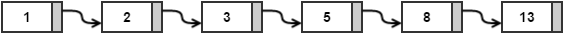
\includegraphics[width=\textwidth]{img/linkedList}
		\caption{Liste chainée ordonnées}
		\label{LinkedList}
	\end{figure}
	
	\subsubsection*{Les alternatives}
	Il existe de nombreuses alternatives aux listes chainées pour trouver un élément plus rapidement: les tables de hashage \cref{hashing}, les arbres binaires \cref{tree}, etc. Mais certaines séquences d'insertions peuvent être catastrophiques. Par exemple, insérer des éléments croissants dans un arbre binaire provoque un rééquilibrage de l'arbre. En revanche, si les éléments sont insérés de façon aléatoire, l'équilibrage devient plus rare.

	Grâce aux probabilités, les \og skip-list \fg{} \cref{skip} bénéficient d'un atout majeur: aucune séquence ne peut provoquer systématiquement le pire scénario. Mieux encore, les skip-lists utilisent des algorithmes plus simples que ses concurrents.
	
	\begin{figure}[h]
		\centering
		\subfloat[Table de hashage] {
			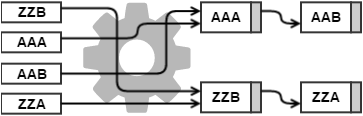
\includegraphics[scale=0.75]{img/hashing}
			\label{hashing}
		}
		\subfloat[Arbre binaire] {
			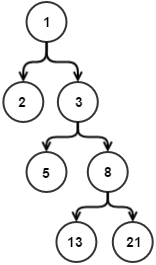
\includegraphics[scale=0.75]{img/tree}
			\label{tree}
		}
		\caption{Différente structures de données}
	\end{figure}
	\begin{figure}
		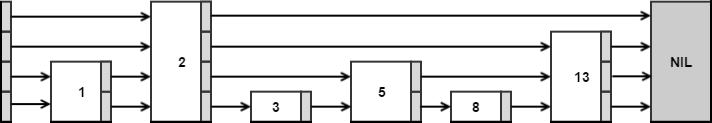
\includegraphics[width=\textwidth]{img/skip}
		\caption{Skip-list}
		\label{skip}
	\end{figure}
	
	\newpage
	\subsection{Skip-List}
	
	
	Tout comme un dictionnaire, une skip-list permet de récupérer la définition d'un terme recherché \textit{(dit clé)}. Cette recherche est rapide, car les éléments \textit{(dit nœud)} présents dans un dictionnaire sont triés et il est possible de commencer une exploration plus approfondie à un endroit précis.
	Une skip-list bénéficie des avantages de la liste chainée, en limitant fortement ses inconvénients. Cette structure de données utilise les chaines de façon parallèle. Une fonction basée sur des probabilités permet de déterminer la hauteur de la chaine. Plus cette hauteur est élevée, moins la liste contient d'éléments. Une couche haute est donc un accès plus rapide vers des éléments plus loin dans la liste.
	
	
	
	Afin d'illustrer la skip-liste, il faut l'imaginer comme un réseau de transport en commun idéal où le temps d'attente des correspondances sont nuls. Un nœud dans la skip-liste est un arrêt obligatoire dans lequel un passager peut changer de moyen de locomotion. La couche la plus basse dans la skip-liste peut-être interprétée comme un bus. Il s'arrête à chacun de ses arrêts prévus, son temps de parcours est très lent. La couche n\degree2, plus rapide, est un métro. La couche n\degree3, un train. Si un passager souhaite aller voir un concert à Bruxelles alors qu'il est à la gare de Charleroi, il ne va pas faire le trajet en bus. Il est tout naturel et plus rapide dans ce cas de prendre dans un premier temps le train, puis le métro afin qu'il se rapproche le plus près possible du concert. Si le dernier arrêt de métro n'a pas permis d'accéder à la salle du concert, seulement dans ce cas le passager doit emprunter le bus.
	
	\begin{figure}[h!]
		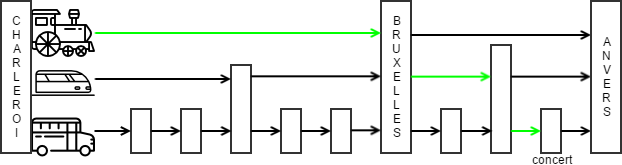
\includegraphics[width=\textwidth]{img/metaphore}
		\caption{Métaphore d'une skip-liste par un réseau de transport en commun}
		\label{skip-meta}
	\end{figure}
	
	\subsubsection*{Définition}
	La hauteur maximale d'une skip-list est définie lors de sa création. Bien qu'il n'y ait pas de taille maximale d'une skip-list, il est conseillé d'utiliser $log_2(n)$ où $n$ est le nombre d'éléments théoriques présents dans la liste.
	
	L'insertion dans la liste utilise une fonction basée sur la probabilité $p$ afin de définir sa hauteur maximale. Si $p$ vaut $\frac{1}{2}$, ça signifie que le nœud une probabilité de $\frac{1}{2}$ d'être de hauteur 2, et une probabilité $\frac{1}{4}$ d'être de hauteur 3. Un nœuds de hauteur $h$ possède $h$ pointeur. Un nœud de hauteur 3 à donc un accès au nœud suivant de hauteur 3, ainsi que celui de hauteur 2 et 1.
	
	En raison des probabilités, les nœuds supérieurs possèdent un pointeur vers un nœud plus avancé dans la liste. Une couche supérieure est donc une voie plus rapide. Ainsi, la couche la plus haute contient les plus grands sauts, et la couche la plus basse permet d'accéder à chacun des éléments.
		
	Le parcours d'une skip-list se fait de haut en bas, et de gauche à droite. Si la clé de l'élément suivant sur une couche est plus grande que celle qu'on recherche, celle-ci continue sur une voie inférieure.	
	
	\begin{figure}[h]
		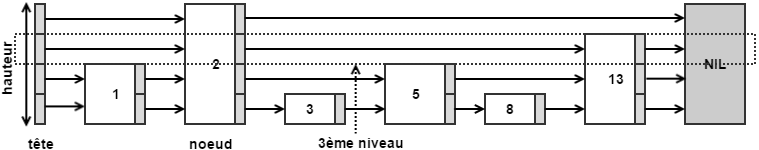
\includegraphics[width=\textwidth]{img/struct}
		\caption{Structure d'une skip-list}
		\label{StructSkip}
	\end{figure}
	
	\subsection{La hauteur}
	La notion de hauteur est très importante dans une skip-liste. En effet, celle-ci permet de définir à combien de nœuds un élément est attaché. Si trop d'éléments possèdent la même hauteur, la recherche devient trop lente.	Cette méthode est définie à l'aide d'une fonction aléatoire. La hauteur ne dépend ni de la clé de l'élément ni de sa valeur. La fonction aléatoire doit être définie pour qu'un élément de hauteur $h$ possède le double de probabilités qu'un élément de hauteur $h+1$. Ainsi, si un nœud de hauteur 1 a une probabilité $p$ de $0.5$ alors le niveau 2 a une probabilité de $0.25$.
		
	\newpage
	\section{Les algorithmes}
	Une skip-list a besoin d'avoir un pointeur vers sa tête $(node* head)$. La liste doit connaitre le nombre de niveaux actuellement utilisé $(level)$. Selon les implémentations, il est possible de définir un nombre de couches maximal $(levelMAX)$. Il est aussi possible de changer le paramètre $(p)$ de probabilité de création d'une nouvelle couche. La variation de ses deux derniers paramètres est étudiée dans le chapitre \nameref{perf}.
	Un nœud contient une clé $key$ , une valeur $value$ ainsi qu'un tableau de pointeur vers les nœuds suivants $forward$. Il n'est pas nécessaire d'enregistrer la hauteur d'un nœud dans celui-ci.
	\lstinputlisting[linerange=BEGINSKStruct-ENDSKStruct]{SkipList/SkipList.h}
	
	L'initiation se fait de la manière suivante:
	\begin{itemize}
		\item La hauteur maximale est déterminée par le nombre d'éléments totaux $(n)$ présents dans la liste. Pour des questions de rapidité, la valeur $log_2(n)$ est recommandée.
		\item Création d'un élément $NIL$ possédant une clé plus grande que le maximum autorisé. Cette élément est aussi appelé \textit{élément bidon}.
		\item Définitions de ses pointeurs $forward$ vers lui-même.
		\item Le nombre de voies actuelles est fixé à 1.
		\item Le pointeur de tête est défini par cet élément $NIL$.
	\end{itemize}
	\emph{La création d'une skip-liste en langage C figure en annexe \ref{SKInit}.}
	
	\begin{figure}[h]
		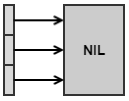
\includegraphics{img/init}
		\caption{Initialisation d'une skip-liste}
		\label{SkipInit}
	\end{figure}
	
	\newpage
	\subsection{La recherche}
	De manière générale, pour rechercher dans une skip-list il suffit de commencer par le niveau le plus haut et d'effectuer une recherche élément par élément. Si l'élément suivant devient plus grand que celui recherché, il suffit alors de descendre d'un niveau dans la liste.
	
	Algorithmiquement parlant, La recherche d'un élément s'exécute de la façon suivante:
	\begin{enumerate}
		\item Commencer l'exploration de la liste par l'élément en tête, et se positionner sur la plus haute voie.
		\item Sur la voie actuelle, regarder la clé de l'élément suivant.
		\item Si elle est plus grande et qu'il existe une voie inférieure, descendre d'une voie.
		\item Sinon aller en 2.
		\item Si la clé de l'élément suivant correspond à celle qui est recherchée: l'élément a été trouvé.
		\item Sinon, l'élément n'a pas été trouvé.
	\end{enumerate}
	
	\emph{L'algorithme écrit en langage C figure en annexe \ref{SKSearch}.}
	
	\subsubsection{Exemples}	
	\paragraph*{Comment rechercher l'élément 8 dans \cref{SkipSearch1}?}
	\begin{itemize}
		\item Se positionner sur la couche la plus haute: La 4ème voie.
		\item 8 est-il plus grand que 2 ? Oui, se positionner sur le nœud 2.
		\item 8 est-il plus grand que $+\infty$ \textit{(NIL)}? Non, descendre sur la 3ème voie.
		\item 8 est-il plus grand que 13  ? Non, descendre sur la 2ème voie.
		\item 8 est-il plus grand que 5 ? Oui, se positionner sur le nœud 5.
		\item 8 est-il plus grand que 13 ? Non, descendre sur la 1ère voie.
		\item 8 est-il plus grand que 8 ? Non, Il n'existe a pas de voie plus basse.
		\item 5 est le dernier nœud parcouru. L'élément suivant sur la voie 1 est 8. 8 est-il l'élément recherché? Oui, la recherche est concluante.
	\end{itemize}
	\begin{figure}[h]
		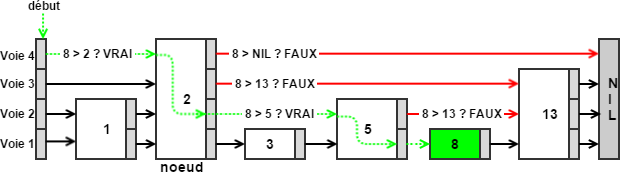
\includegraphics[width=\textwidth]{img/search}
		\caption{Recherche de l'élément 8 dans une skip-liste}
		\label{SkipSearch1}
	\end{figure}
	
	\newpage
	\paragraph*{Comment rechercher l'élément 9 dans \cref{SkipSearch2}?}
	
	\begin{itemize}
		\item Se positionner sur la couche la plus haute: La 4ème voie.
		\item 8 est-il plus grand que 2 ? Oui, se positionner sur le nœud 2.
		\item 8 est-il plus grand que $+\infty$ \textit{(NIL)}? Non, descendre sur la 3ème voie.
		\item 8 est-il plus grand que 13  ? Non, descendre sur la 2ème voie.
		\item 8 est-il plus grand que 5 ? Oui, se positionner sur le nœud 5.
		\item 8 est-il plus grand que 13 ? Non, descendre sur la 1ère voie.
		\item 8 est-il plus grand que 8 ? Non, Il n'existe a pas de voie plus basse.
		\item 5 est le dernier nœud parcouru. L'élément suivant sur la voie 1 est 9. 9 est-il l'élément recherché? Non, la recherche est infructueuse.
	\end{itemize}
	\begin{figure}[h]
		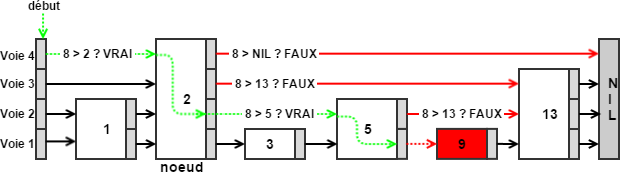
\includegraphics[width=\textwidth]{img/search2}
		\caption{Recherche de l'élément 9 dans une skip-liste}
		\label{SkipSearch2}
	\end{figure}
	
	
	\newpage
	\subsection{L'insertion}
	L'insertion d'une entrée dans une skip-list est essentiellement la même chose que la recherche. A l'exception qu'un tableau $update$, de taille identique à la hauteur de la liste, est utilisé pour mémoriser les pointeurs chaque l'élément avant de descendre d'un niveau. Ce tableau est utilisé pour mettre à jour les liens nécessaires pour que la structure de donnée reste cohérente.
	
	Algorithmiquement parlant, l'insertion d'un élément dans une skip-liste s'effectue de la façon suivante:
	\begin{enumerate}
		\item Commencer l'exploration de la liste par l'élément en tête, et se positionner sur la plus haute voie.
		\item Sur la voie actuelle, regarder la clé de l'élément suivant.
		\item Si elle est plus grande et qu'il existe une voie inférieure, marquer ce pointeur. Puis, descendre d'une voie.
		\item Sinon aller en 2.
		\item Si la clé de l'élément suivant correspond à celle qui est recherchée: modifier la valeur de l'élément par celle de la valeur à insérer. \textbf{FIN}.
		\item Sinon, appeler la fonction de probabilité pour récupérer sa valeur $n$.
		\item Si $n$ est plus grand que la hauteur $h$ de la liste, mettre à jour les pointeurs supérieurs à $h$ vers $NIL$. Ensuite, définir la hauteur maximum actuelle $h$ à $n$.
		\item Créer le nœud $x$ de hauteur $n$.
		\item Pour chaque voie de $1$ à $n$.
		\item Mettre à jour les pointeurs de $x$ vers l'élément suivant de l'élément marqué de cette voie.
		\item Mettre à jour les pointeurs de l'élément marqué de cette voie vers $x$.
		\item \textbf{FIN}.
	\end{enumerate}
	\emph{L'algorithme écrit en langage C est présenté en annexe \ref{SKInsert}.}
	
	\newpage
	\subsubsection{Exemples}	
	\paragraph*{Comment insérer l'élément 8 dans \cref{SkipInsert1}?}
	\begin{itemize}
		\item Se positionner sur la couche la plus haute: La 4ème voie.
		\item 8 est-il plus grand que 2 ? Oui, se positionner sur le nœud 2.
		\item 8 est-il plus grand que $+\infty$ \textit{(NIL)}? Enregistrer ce lien en mémoire, puis descendre sur la 3ème voie.
		\item 8 est-il plus grand que 13  ? Enregistrer ce lien en mémoire, puis descendre sur la 2ème voie.
		\item 8 est-il plus grand que 5 ? Oui, se positionner sur le nœud 5.
		\item 8 est-il plus grand que 13 ? Enregistrer ce lien en mémoire, puis descendre sur la 1ère voie.
		\item 8 est-il plus grand que 8 ? Enregistrer ce lien en mémoire, Il n'existe a pas de voie plus basse.
		\item 5 est le dernier nœud parcouru. L'élément suivant sur la voie 1 est 8. 8 est-il l'élément recherché? Non, on créer un nouvel élément. Générer une hauteur aléatoire: hauteur 1.
		\item Ajouté un lien du nouvel élément 8 en voie 1. Ce lien doit pointer vers l'élément du lien enregistré à cette même voie. Il s'agit de l'élément 13.
		\item Modifier ce lien enregistré en voie 1 (de l'élément 5 vers l'élément 13) pour qu'il pointe vers ce nouvel élément 8.
		\item FIN.
	\end{itemize}
	\begin{figure}[h]
		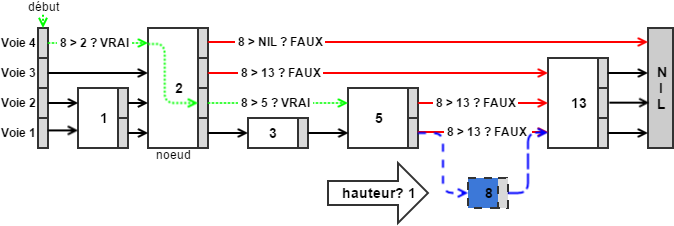
\includegraphics[width=\textwidth]{img/insert}
		\caption{Insertion dans une skip-liste}
		\label{SkipInsert1}
	\end{figure}
	
	\newpage
	\paragraph*{Comment insérer l'élément 5 dans \cref{SkipInsert1}?}
	\begin{itemize}
		\item Se positionner sur la couche la plus haute: La 4ème voie.
		\item 5 est-il plus grand que 2 ? Oui, se positionner sur le nœud 2.
		\item 5 est-il plus grand que $+\infty$ \textit{(NIL)}? Enregistrer ce lien en mémoire, puis descendre sur la 3ème voie.
		\item 5 est-il plus grand que 13 ? Enregistrer ce lien en mémoire, puis descendre sur la 2ème voie.
		\item 5 est-il plus grand que 13 ? Enregistrer ce lien en mémoire, puis descendre sur la 1ère voie.
		\item 5 est-il plus grand que 3 ? Oui, se positionner sur le nœud 3.
		\item 5 est-il plus grand que 8 ? Enregistrer ce lien en mémoire, Il n'existe a pas de voie plus basse.
		\item 5 est le dernier nœud parcouru. L'élément suivant sur la voie 1 est 8. 8 est-il l'élément recherché? Non, on créer un nouvel élément. Générer une hauteur aléatoire: hauteur 2.
		\item Ajouté un lien du nouvel élément 5 en voie 1. Ce lien doit pointer vers l'élément du lien enregistré à cette même voie. Il s'agit de l'élément 8.
		\item Modifier ce lien enregistré en voie 1 (de l'élément 3 vers l'élément 8) pour qu'il pointe vers ce nouvel élément 5.
		\item Ajouté un lien du nouvel élément 5 en voie 2. Ce lien doit pointer vers l'élément du lien enregistré à cette même voie. Il s'agit de l'élément 13.
		\item Modifier ce lien enregistré en voie 2 (de l'élément 2 vers l'élément 13) pour qu'il pointe vers ce nouvel élément 5.
		\item FIN.
	\end{itemize}
	\begin{figure}[h]
		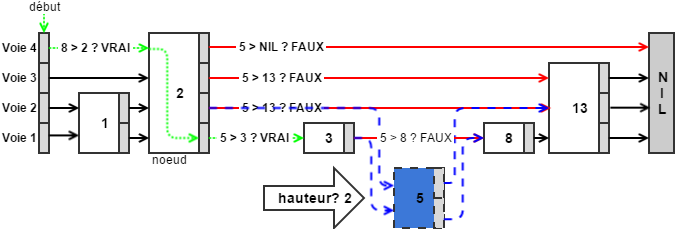
\includegraphics[width=\textwidth]{img/insert2}
		\caption{Insertion dans une skip-liste}
		\label{SkipInsert2}
	\end{figure}
	
	\newpage
	\subsection{La suppression}
	La suppression d'un élément dans une skip-liste s'effectue de la façon suivante:
	\begin{enumerate}
		\item Commencer l'exploration de la liste par l'élément en tête, et se positionner sur la plus haute voie.
		\item Sur la voie actuelle, regarder la clé de l'élément suivant.
		\item Si elle est plus grande et qu'il existe une voie inférieure, marquer ce nœud. Puis, descendre d'une voie.
		\item Sinon aller en 2.
		\item Si la clé de l'élément suivant ne correspond pas à celle qui est recherchée, \textbf{FIN}.
		\item Sinon pour chaque niveau de l'élément trouvé $x$, mettre à jour les pointeurs de l'élément marqué de cette voie vers l'élément suivant de $x$.
		\item Supprimer $x$.
		\item Si l'élément de tête de la hauteur actuelle de la liste pointe vers $NIL$, diminuer la hauteur actuelle de la liste de 1.
		\item Sinon, \textbf{FIN}.
		\item Si la hauteur est plus grande que 1, aller en 8.
	\end{enumerate}
	\emph{L'algorithme écrit en langage C figure en annexe \ref{SKDelete}.}
	\begin{center}
		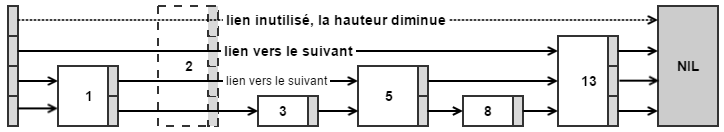
\includegraphics[width=\textwidth]{img/delete}
	\end{center}
	
	\newpage
	\section{Analyse des performances}\label{perf}
	La caractéristique majeure de la skip-list est l'aléatoire. L'insertion d'un élément nouveau utilise une hauteur qui est déterminée par le hasard. De ce fait, une même séquence produira une liste différente. Cela a comme conséquence qu'aucune séquence prédéterminée de nombres ne peut produire une dégradation des performances, contrairement aux arbres binaires qui eux doivent être constamment rééquilibrés.
	
	De par sa nature probabiliste, on suppose que l'utilisateur n'aura pas un comportement à vouloir dégénéré volontairement la liste. C'est-à-dire que les performances peuvent être dégradées en retirant consciemment les éléments après avoir inspecté leur hauteur. Si l'utilisateur supprime tous les nœuds de hauteur $h>1$, le pire scénario de la skip-list équivaut à une liste chainée classique.
	
	Le temps requis pour exécuter l'insertion et la suppression dans une skip-list est prédominé par le temps de la recherche d'un élément. Ces deux derniers n'ont qu'un cout supplémentaire constant par rapport à la hauteur de la liste; alors que le cout de la recherche est proportionnel à la longueur du chemin à parcourir.
	
	
	\subsection{Analyse pour $p=\frac{1}{2}$}
	Pour une variable aléatoire $p=\frac{1}{2}$ et une skip-list de taille infinie, celle-ci tend à ce que chacun des niveaux possèdes $\frac{1}{2}$ moins d'éléments. Ainsi, le niveau 1 contient $n$ élément, le niveau 2 $\frac{n}{2}$, le niveau 3 $\frac{n}{4}$, ..., un élément à hauteur $h$: $\frac{n}{{2}^{h-1}}$. Par conséquent, le nombre total de liens dans une skip-list équivaut à \[n+\frac{n}{2}+\frac{n}{4}+\frac{n}{8}+\dots = \sum_{h=1}^{+\infty}\frac{n}{{2}^{h-1}}=2n\] Ce qui signifie qu'en moyenne un élément dans une skip-list possède 2 liens. Vu que la recherche se fait de haut en bas et de gauche à droite, chaque clé examinée à un niveau précis ($i$) ne peut pas appartenir à un niveau supérieur ($i+1$).
	De ce fait, on peut déduire qu'en moyenne le nombre de fois que l'on avance dans la liste à un niveau précis équivaut au nombre de liens divisé par le nombre d'éléments, soit $\frac{2n}{n}=2$.
	
	\newpage
	La probabilité qu'un élément soit de hauteur $i$ est de ${p^{i}} = \frac{1}{2^{i}} $. Le facteur $p$ est constant ($\frac{1}{2}$), la probabilité de la hauteur des clés est équiprobable. Si l'on additionne la probabilité de hauteur chacune des clés de la skip-list, et que l'on prend $h$ comme hauteur de la liste, on déduit la formule suivante.
	\[
		\frac{1}{{2}^{1}}+\frac{1}{{2}^{2}}+\frac{1}{{2}^{3}}+\dots+\frac{1}{{2}^{h}}
		= \sum _{i=1}^{h} ({\frac{1}{2}})^{i}
	\]
	Cette hauteur, il est possible de l'estimer. Si $h$ tend vers l'infini, la série converge vers 1. Ce qui as comme conséquence:
	\[
		n{(\frac{1}{2})}^{h} = 1
		\iff {(\frac{1}{2})}^{h}=\frac{1}{n}
		\iff h = \log_{\frac{1}{2}}(\frac{1}{n})
		\iff h = \log_{2}(n)
	\]
	
	L'algorithme de recherche effectue possède 2 boucles imbriquées. La boucle la plus profonde permet d'avancer de gauche à droite dans la liste. Pour $p=\frac{1}{2}$, en moyenne celle-ci avance de $2$. La boucle supérieure quant à elle varie selon la hauteur de la liste. La hauteur est estimée, avec une forte probabilité, à $\log_{2} n $. Si l'on combine les 2 estimations, nous avons donc une forte probabilité que la recherche s'effectue en $\log_{2}( 2n )$ opérations, soit $\mathcal{O}(log(n))$.
	
	
	\subsubsection{Généralisation}
	
	Le raisonnement utilisé précédemment pour $p=\frac{1}{2}$ reste valable quelque soit la valeur de $p$, voir \cref{recap}. Le raisonnement qui effectue une sommation servant au calcule de lien dans une liste convergera vers $\frac{n}{p}$. Par contre, la somme des probabilités ($p^1 + p^2 + p^3 + ... + p^k$), converge toujours vers $\frac{p}{1-p}$. 
	 	
	 \begin{table}[h]
	 \begin{tabular}{|l|c|c|}
	 	\hline
	 	Scénario & attendu & pire \\
	 	\hline
	 	Nombre d'élément & $n$ & $n$ \\ 
	 	\hline
	 	Hauteur & $log_{\frac{1}{p}} n$ & $\infty$ \\ 
	 	\hline
	 	Nombre de lien & $n/p$ & $n*h$ \\ 
	 	\hline
	 	Recherche & $\mathcal{O}(\log n)$ & $\mathcal{O}(n)$ \\ 
	 	\hline
	 	Insertion & $\mathcal{O}(\log n)$ & $\mathcal{O}(n)$ \\
	 	\hline
	 	Suppression & $\mathcal{O}(\log n)$ & $\mathcal{O}(n)$\\
	 	\hline
	 \end{tabular}
	 \caption{Tableau récapitulatif}
	 \label{recap}
	 \end{table}
	 
	 \subsubsection{Le pire cas}
	 	
	 Les ordinateurs ne possèdent pas une mémoire infinie. Par conséquent, il est impossible d'ajouter une infinité d'éléments. C'est pourquoi à la création d'une skip-list, la hauteur maximale est bornée par la formule du cas attendu avec une forte probabilité. Le pire scénario de hauteur infinie est donc impossible. Dans le cas très improbable que chacun des éléments de la skip-list soit à cette hauteur maximale, nous avons une recherche en $n*h$: soit $\mathcal{O}(n)$. 
	 	
	 De façon générale, avec une constance $c>1$ $h$ est plus grande que $c log n$ avec une probabilité d'au plus $\frac{1}{n^{c-1}}$. En d'autres mots, la probabilité que $h$ soit plus petit que $c log n$ est d'au moins $1-\frac{1}{n^{c-1}}$. Par conséquent, avec une forte probabilité, la hauteur d'une skip-liste est bien d'ordre $\mathcal{O}(log n)$. Par exemple: si $n=1000$, la probabilité est d'une sur un million.
	
	
	\subsection{Expérimentation}
	
	Les expérimentations suivantes ont été réalises sur un ordinateur Windows 10 64 bits possédant un AMD FX 8350 et 16Gb de RAM. Les tests ont été lancés $10^5$ fois, les résultats présent sont la moyenne des tests.
	\newline
	
	Afin de vérifier que le $p$ à bien l'effet voulu, il suffit de compter le nombre de lien existant à chaque niveau. S'il y a $n$ éléments à la hauteurs 1, on s'attend à obtenir $np$ éléments de hauteur 2 avec une forte probabilité.

	Dans les faits, en essayant différentes valeurs pour une skip-list de 1000 éléments, on  peut obtenir les résultats présents dans \cref{tbRes1}. Le résultat obtenu, correspond à notre espérance: $p$ influence correctement la hauteur de la liste, et par conséquent sont poids.
	\begin{table}[h]
		\resizebox{\columnwidth}{!}{
		\begin{tabular}{|c|r|r|r|r|r|r|r|r|r|r|r|r|r|r|}
			\hline
			\backslashbox{p}{h} & 1 & 2 & 3 & 4 & 5 & 6 & 7 & 8 & 9 & 10 & 11 & 12 & 13 & 14 \\
			\hline
			4/5 & 1001 & 800,98 & 640,98 & 513,02 & 410,69 & 328,76 & 263,2 & 210,79 & 168,81 & 135,26 & 108,41 & 86,94 & 69,73 & 55,99 \\
			3/4 & 1001 & 751,05 & 563,5 & 422,86 & 317,35 & 238,26 & 178,93 & 134,44 & 101,08 & 76,05 & 57,29 & 43,22 & 32,68 & 24,76 \\
			2/3 & 1001 & 667,63 & 445,44 & 297,22 & 198,46 & 132,59 & 88,74 & 59,51 & 40,02 & 27 & 18,33 & 12,55 & 8,7 & 6,13 \\
			3/5 & 1001 & 601,03 & 361,05 & 217,06 & 130,64 & 78,77 & 47,66 & 28,99 & 17,79 & 11,08 & 7,04 & 4,59 & 3,06 & 2,03 \\
			1/2 & 1001 & 500,99 & 251,01 & 126,04 & 63,53 & 32,27 & 16,62 & 8,81 & 4,88 & 2,81 & 0 & 0 & 0 & 0 \\
			2/5 & 1001 & 401,01 & 161,02 & 65,02 & 26,61 & 11,24 & 5,08 & 2,45 & 0 & 0 & 0 & 0 & 0 & 0 \\
			1/3 & 1001 & 334,33 & 112,1 & 38,03 & 13,34 & 5,09 & 0 & 0 & 0 & 0 & 0 & 0 & 0 & 0 \\
			1/4 & 1001 & 250,9 & 63,5 & 16,62 & 4,9 & 0 & 0 & 0 & 0 & 0 & 0 & 0 & 0 & 0 \\
			1/5 & 1001 & 201,05 & 41,03 & 9,01 & 0 & 0 & 0 & 0 & 0 & 0 & 0 & 0 & 0 & 0 \\
			\hline
		\end{tabular}
		}
		\caption{Le nombre de lien par niveau en fonction de $p$}
		\label{tbRes1}
	\end{table}
	
	
	
	\begin{appendices}
	\newpage
	\section{Représentation d'une Skip-List en langage C}
	\subsection{Initiation}\label{SKInit}
	\lstinputlisting[linerange=BEGINSKInit-ENDSKInit]{SkipList/SkipList.c}
	\subsection{Fonction aléatoire}\label{SKRandom}
	\lstinputlisting[linerange=BEGINSKRandom-ENDSKRandom]{SkipList/SkipList.c}

	\subsection{Recherche}\label{SKSearch}
	\lstinputlisting[linerange=BEGINSKSearch-ENDSKSearch]{SkipList/SkipList.c}

	\subsection{Insertion}\label{SKInsert}
	\lstinputlisting[linerange=BEGINSKInsert-ENDSKInsert]{SkipList/SkipList.c}
	
	\subsection{Suppression}\label{SKDelete}
	\lstinputlisting[linerange=BEGINSKDelete-ENDSKDelete]{SkipList/SkipList.c}
	\newpage
	\end{appendices}
	
	
	@online{1,
		author = {Patrice Roy},
		title = {Skip Lists},
		date = {27/02/2016},
		url = {http://h-deb.clg.qc.ca/Sujets/Structures-donnees/SkipLists.html},
	}
	@online{2,
		author = {Sylvie Hamel},
		title = {Dictionnaires ordonnés et “Skip List”},
		date = {25/02/2016},
		url = {http://www.iro.umontreal.ca/~hamelsyl/SkipList.pdf},
	}
	
\end{document} 